\subsection{Area between two graphs}

On the interval $[0,1]$, the graph of $y=x$ lies above the graph of $y=x^2$. The area between them is
\[
\int_0^1 \bigl(x-x^2\bigr)\,dx.
\]

\begin{center}
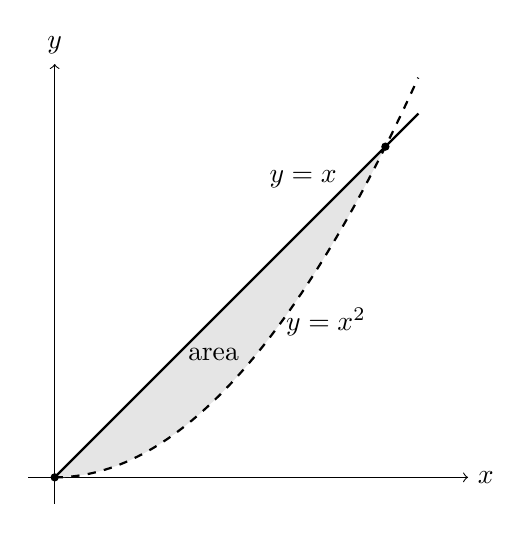
\begin{tikzpicture}[x=4.2cm,y=4.2cm]
  \draw[->] (-0.08,0) -- (1.25,0) node[right] {$x$};
  \draw[->] (0,-0.08) -- (0,1.25) node[above] {$y$};
  \fill[gray!20] plot[domain=0:1,samples=80] (\x,\x)
    -- plot[domain=1:0,samples=80] (\x,{\x*\x}) -- cycle;
  \draw[thick,domain=0:1.1,samples=2] plot (\x,\x);
  \draw[thick,dashed,domain=0:1.1,samples=80] plot (\x,{\x*\x});
  \fill (0,0) circle (1.5pt);
  \fill (1,1) circle (1.5pt);
  \node[anchor=west] at (0.62,0.9) {$y=x$};
  \node[anchor=west] at (0.67,0.47) {$y=x^2$};
  \node at (0.48,0.37) {area};
\end{tikzpicture}
\end{center}

\begin{interpretationbox}[Top minus bottom]
A vertical strip has height equal to the upper function minus the lower function. Integrating that difference adds the strip areas across the interval.
\end{interpretationbox}
